\section{KV-Direct 操作原语}
\label{kvdirect:sec:architecture}
\label{kvdirect:sec:kv-operations}

KV-Direct 将远程直接内存访问(RDMA)原语扩展到 \textit {远程直接键值访问},如表 \ref {kvdirect:tab:kv-operations} 所述。
客户端将\textit {KV-Direct 操作}发送到键值存储服务器,而可编程网卡处理请求并发送回结果,绕过CPU。
键值存储服务器上的可编程网卡是一个重新配置为\textit {键值处理器}的FPGA。

除了表 \ref {kvdirect:tab:kv-operations} 顶部所示的标准键值存储操作外,KV-Direct还支持两种类型的向量运算:
将标量发送到服务器上的网卡,网卡将更新应用于向量中的每个元素;或者向服务器发送一个向量,并且网卡逐个元素地更新原始向量。
此外,KV-Direct支持用户定义的更新功能,作为原子操作的概括。
更新功能需要在执行前预先注册并编译为硬件逻辑。
使用用户定义的更新功能的键值操作类似于\textit {动态消息}(active message)\cite {eicken1992active},从而节省了通信和同步成本。


\begin{table}
\centering
\caption{KV-Direct 操作。}
\label{kvdirect:tab:kv-operations}
\small
\begin{tabular}{p{.4\textwidth}|p{.5\textwidth} }
\toprule
get ($k$) $\rightarrow v$ & 获取键 $k$ 的值。 \\
\midrule
put ($k, v$) $\rightarrow$ bool & 插入或替换 $(k, v)$ 对。 \\
\midrule
delete ($k$) $\rightarrow$ bool & 删除键 $k$。 \\
\midrule
\midrule
update{\_}scalar2scalar ($k, \Delta, \lambda(v, \Delta) \rightarrow v$) $\rightarrow v$ & 原子更新键 $k$,使用函数 $\lambda$,作用于 $\Delta$ 上,返回原始值。\\
\midrule
update{\_}scalar2vector ($k, \Delta, \lambda(v, \Delta) \rightarrow v$) $\rightarrow [v]$ & 原子更新键 $k$ 中的所有元素,使用函数 $\lambda$ 和标量 $\Delta$,返回原始向量。 \\
\midrule
update{\_}vector2vector ($k, [\Delta], \lambda(v, \Delta) \rightarrow v$) $\rightarrow [v]$ & 原子更新键 $k$ 中的所有元素,使用函数 $\lambda$,基于向量 $[\Delta]$ 中的对应元素,并返回原始向量。 \\
\midrule
reduce ($k, \Sigma, \lambda(v, \Sigma) \rightarrow \Sigma$) $\rightarrow \Sigma$ & 把向量 $k$ 归约成一个标量,使用函数 $\lambda$,并返回归约结果 $\Sigma$。 \\
\midrule
filter ($k, \lambda(v) \rightarrow$ bool) $\rightarrow [v]$ & 在向量 $k$ 中筛选元素,使用函数 $\lambda$,并返回筛选后的向量。 \\
\bottomrule
\end{tabular}
\end{table}

当对键执行向量操作更新(update),归约(reduce)或过滤(filter)时,其值被视为固定位宽元素的数组。
每个函数 $\lambda$ 对向量中的一个元素,客户端指定的参数 $\Delta$ 和/或初始值 $\Sigma$ 进行归约操作。
KV-Direct开发工具链多次复制$\lambda$以利用FPGA中的并行性并将计算吞吐量与PCIe吞吐量相匹配,然后使用高级综合(HLS)工具将其编译为可重新配置的硬件逻辑\cite {aoc} 。
HLS工具自动提取复制函数中的数据依赖性,并生成完全流水线的可编程逻辑。
在执行键值存储客户端之前,键值存储服务器上的可编程网卡应加载包含展开的$\lambda$的硬件逻辑。

使用用户定义函数的更新操作能够对向量值进行常规流处理。
例如,网络处理应用程序可以将该向量解释为用于网络功能的分组流\cite{li2016clicknp}或用于分组事务的一堆状态\cite {sivaraman2016packet}。
完全在可编程网卡中的单对象事务处理也是可能的,例如,在TPC-C基准中包围S\_QUANTITY \cite {council2010tpc}。
向量归约操作支持PageRank \cite {page1999pagerank}中的邻居权重累积。
可以使用向量过滤操作来获取稀疏向量中的非零值。

\section{键值处理器}
\label{kvdirect:sec:kv-processor}

\begin{figure}[htbp]
\centering
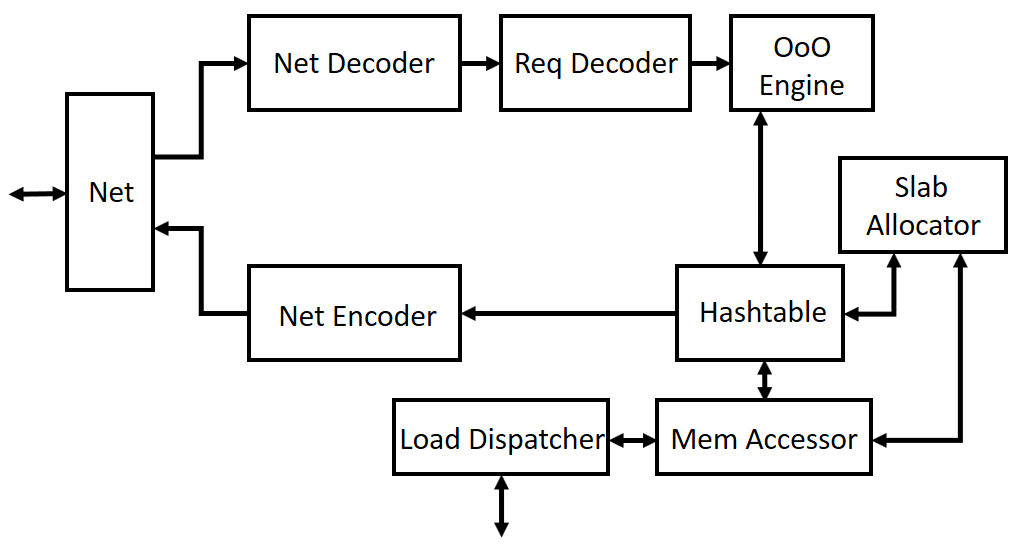
\includegraphics[width=0.7\textwidth,page=1]{processor_architecture.PNG}
\caption{键值处理器架构。}
\label{kvdirect:fig:kvprocessor-arch}
\end{figure}

如图\ref {kvdirect:fig:kvprocessor-arch}所示,键值处理器从板载网卡接收数据包,解码向量操作并缓冲保留站中的键值操作(\S \ref {kvdirect:sec:ooo})。
接下来,乱序执行引擎(\S \ref {kvdirect:sec:ooo})从保留站向操作解码器发出独立的键值操作。
根据操作类型,键值处理器查找哈希表(\S \ref {kvdirect:sec:hashtable})并执行相应的操作。
为了最小化内存访问次数,较小的键值对在哈希表中内联(inline)存储,其他的键值对存储在slab内存分配器(\S \ref {kvdirect:sec:slab})的动态分配内存中。
哈希索引和slab分配的内存都由统一的内存访问引擎(\S \ref {kvdirect:sec:dram-cache})管理,它通过PCIe DMA访问主机内存并缓存部分主机内存。板载DRAM。
在键值操作完成之后,结果被发送回无序执行引擎(\S \ref {kvdirect:sec:ooo})以在保留站中找到并执行匹配的键值操作。

正如\S \ref {kvdirect:sec:challenge}中所讨论的,PCIe操作吞吐量的稀缺性要求键值处理器在DMA访问上节俭。
对于GET操作,至少需要读取一次内存。
对于PUT或DELETE操作,对于哈希表,一次读取和一次写入最小。
基于日志的数据结构可以实现每个PUT一次写入,但它牺牲了GET性能。
KV-Direct仔细设计哈希表,以便在每次查找和插入时实现接近理想的DMA访问,以及内存分配器。每次动态内存分配平摊下来,只需不到0.1次DMA操作。

\subsection{哈希表}
\label{kvdirect:sec:hashtable}

为了存储可变大小的键值,键值存储分为两部分。 第一部分是哈希索引(图\ref {kvdirect:fig:hashtable}),它包含固定数量的\textit {哈希桶}。 每个哈希桶包含几个\textit {哈希槽}和一些元数据。 内存的其余部分是动态分配的,由slab分配器(\S \ref {kvdirect:sec:slab})管理。
初始化时配置的\textit {哈希索引比率}确定为哈希索引分配的内存百分比。
哈希索引比率的选择将在\S \ref {kvdirect:sec:hashtable-eval}中讨论。


\begin{figure}[htbp]
	\centering
	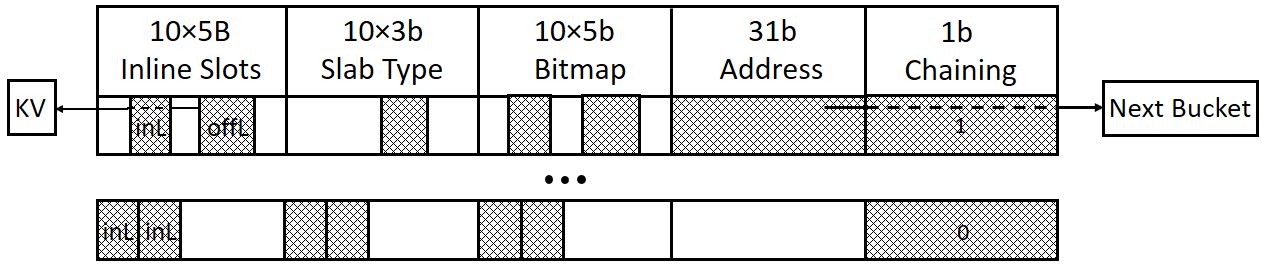
\includegraphics[width=1.0\textwidth,page=1]{hashline.PNG}
	\caption{哈希索引结构。 每行是一个哈希桶,包含10个哈希槽,每个哈希槽3位板内存类型,一个位图标记内联键值对的开始和结束,以及指向哈希冲突下一个链接桶的指针。}
	\label{kvdirect:fig:hashtable}
\end{figure}


%\textbf{Hash Table.}
%Each bucket includes 10 hash slots, 3b type code per slot, 50b metadata, plus 31b address and a valid bit of the next chained bucket, as shown in Figure~\ref{kvdirect:fig:hashtable}.
%For offline 键值s, each hash slot needs to store 31b of address, 9b of secondary hash and 3b type code for the slab size.
%For inline 键值s, to mark the begin and end of each hash slot, as well as the separation between inline key and value, the information is encoded in a 50b metadata corresponding to 50 bytes of hash slots.
%The inline keys and secondary hashes of offline keys in all hash slots are compared in parallel, and the first match is found.

每个哈希槽包括指向动态分配的存储器中的键值数据的指针和辅助哈希。
辅助哈希是一种启用并行内联检查的优化。始终检查键以确保正确性,但需要额外的一次内存访问。
假设主机内存中的64~GiB 键值存储和32字节分配粒度(内部碎片和分配元数据开销之间的权衡),指针需要31位。
9位的二级哈希给出1/512误报可能性。
累积地,哈希槽大小是5个字节。
为了确定哈希桶大小,需要在每个桶的哈希槽数和DMA吞吐量之间进行权衡。
图\ref {kvdirect:fig:dma-tput}表明DMA读取吞吐量低于64B粒度受DMA引擎中PCIe延迟和并行性的约束。
由于哈希冲突的可能性增加,小于64B的桶大小是次优的。
另一方面,将桶大小增加到64B以上会降低哈希查找吞吐量。
因此桶大小选择为64字节。

\textit {键值大小}是指键和值的总大小。
小于阈值的键值在哈希索引中内联(inline)存储,以保存对获取键值数据的额外存储器访问。
内联键值可以跨越多个哈希槽,其指针和二级哈希字段被重新用于存储键值数据。
内联所有可装入铲斗的键值可能不是最佳选择。
为了最小化平均访问时间,假设可以同等地访问越来越小的键,则更希望内联小于\textit {内联阈值}的键值。
为了量化所有桶中使用的桶的部分,本章使用\textit {内存利用率}而不是负载率(load factor),因为它更多地涉及可以适合固定内存量的键值的数量。
如图\ref {kvdirect:fig:inline-offline}所示,对于某个内联阈值,由于更多的哈希冲突,平均内存访问计数随内存利用率的增加而增加。
较高的内联阈值显示内存访问计数的更陡峭的增长曲线,因此可以找到最佳内联阈值以最小化在给定内存利用率下的内存访问。
与哈希索引比率一样,也可以在初始化时配置内联阈值。


\begin{figure}[htbp]
	\centering
	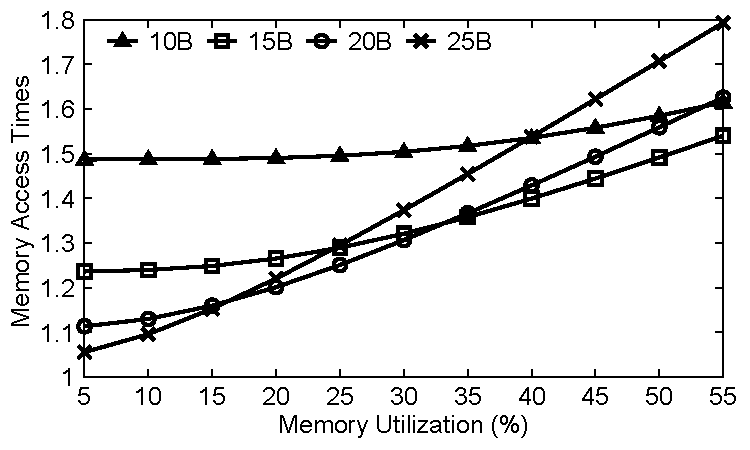
\includegraphics[width=0.6\textwidth]{inline_thresh.pdf}
	\caption{不同内联阈值下的平均内存访问次数和内存利用率。}
	\label{kvdirect:fig:inline-offline}
\end{figure}


当存储桶中的所有插槽都已填满时,有几种解决方案可以解决哈希冲突。
Cuckoo哈希\cite {pagh2004cuckoo}和跳房子哈希(Hopscotch Hash)\cite {herlihy2008hopscotch}通过在插入过程中移动占用的插槽来保证恒定时间查找。
但是,在写入密集型工作负载中,高负载率下的内存访问时间会经历大的波动。
线性探测可能受到主群集的影响,因此其性能对哈希函数的均匀性敏感。
为此,选择\textit {拉链法}来解决哈希冲突,这会平衡查找和插入,同时对哈希群集更加健壮。

%In KV-Direct, we measure memory utilization instead of load factor, because chaining has dynamic size and that we care more about the overall storage efficiency counting all indexing, metadata and memory fragmentation overhead.
%Clearly, small 键值s cause lower memory utilization due to metadata overhead.
%The optimal hash index ratio is chosen at initialization time according to workload to balance average access time and memory utilization.

\label{kvdirect:sec:hashtable-eval}

哈希表设计中有两个自由参数:(1)内联阈值,(2)整个内存空间中哈希索引的比率。
如图\ref {kvdirect:fig:optimize_fix_mem}所示,当哈希索引比率增长时,可以内联存储更多的键值对,从而产生更低的平均内存访问时间。
图\ref {kvdirect:fig:optimize_fix_ratio}显示了随着使用更多内存而增加的内存访问量。
如图\ref {kvdirect:fig:hashline-ratio}所示,最大可实现内存利用率在较高哈希索引比率下下降,因为可用于动态分配的内存较少。
因此,为了在给定的存储器大小中容纳整个语料库,哈希索引比率具有上限。
本节选择此上限并获得最小的平均内存访问时间,如图\ref {kvdirect:fig:hashline-ratio}中的虚线所示。


\begin{figure}[htbp]
	\subfloat[固定内存利用率 0.5。\label{kvdirect:fig:optimize_fix_mem}]
	{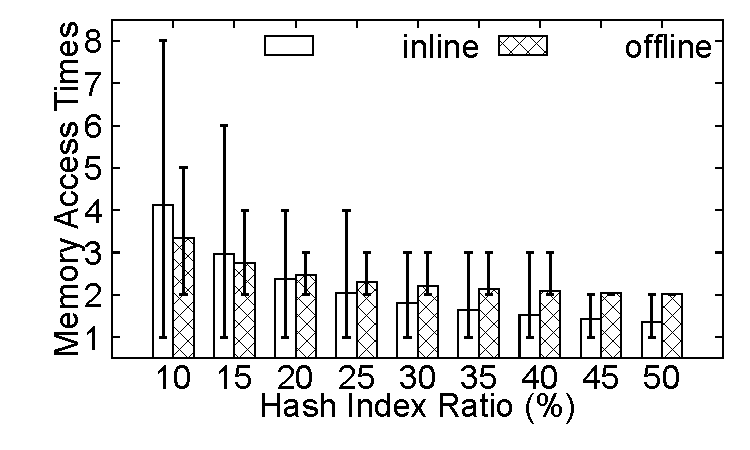
\includegraphics[width=.5\textwidth,page=1]{fix_mem.pdf}}
	\subfloat[固定哈希索引率 0.5。\label{kvdirect:fig:optimize_fix_ratio}]
	{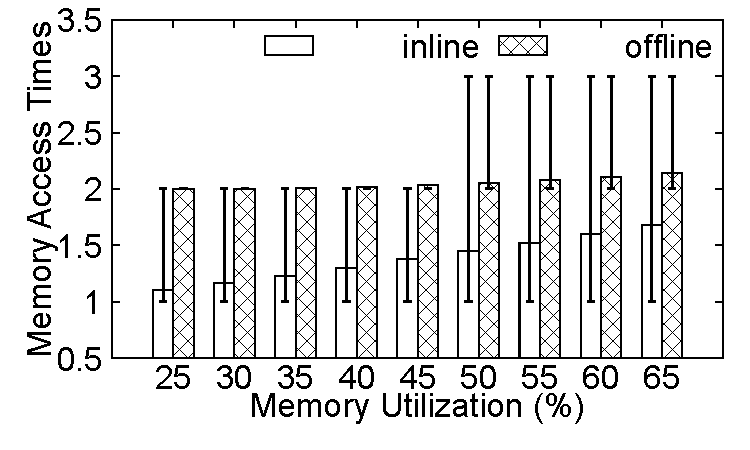
\includegraphics[width=.5\textwidth,page=1]{fix_ratio.pdf}}
	\caption{不同内存利用率或哈希索引率下的内存占用。}
	\label{kvdirect:fig:memory-access-count}
\end{figure}

\begin{figure}[htbp]
	\centering
	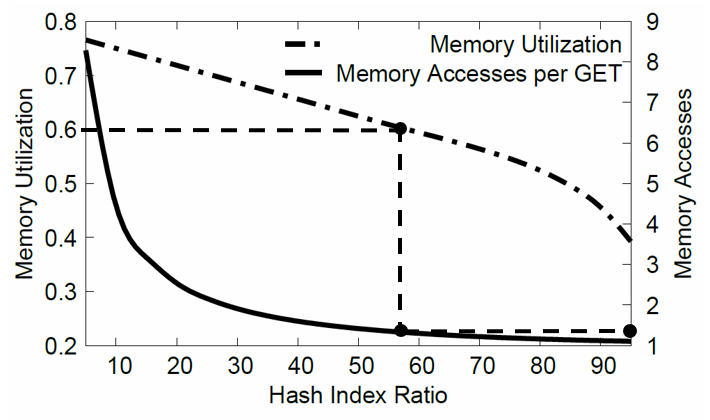
\includegraphics[width=0.6\textwidth,page=1]{optimize.png}
	\caption{如何在给定内存利用率需求和键值大小的情况下决定最优哈希索引率。}
	\label{kvdirect:fig:hashline-ratio}
\end{figure}

图\ref {kvdirect:fig:mem-access-tput} 绘制了三种可能的哈希表设计的每个GET和PUT操作的内存访问次数:在KV-Direct中链接,MemC3中的桶式布谷鸟哈希(bucketized Cuckoo Hash)\cite {fan2013memc3} 和FaRM \cite {dragojevic2014farm} 中的链式关联(chain associative)跳房子哈希(Hopscotch Hash)。
对于KV-Direct,针对给定的键值大小和内存利用率要求,为内联阈值和哈希索引比率做出最佳选择。
对于布谷鸟和跳房子哈希,假设键是内联的并且可以并行比较,而值存储在动态分配的板中。
由于MemC3和FaRM的哈希表不能支持10B 键值大小超过55%的内存利用率,图\ref {kvdirect:fig:mem-access-10-get}和图\ref {kvdirect:fig:mem-access-10-put}仅显示KV-Direct的性能。


\begin{figure}[htbp]
	\centering
	\subfloat[10B GET.\label{kvdirect:fig:mem-access-10-get}]
	{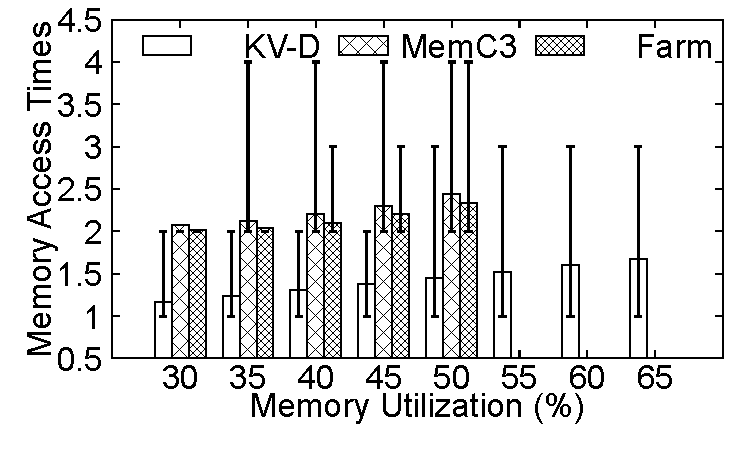
\includegraphics[width=.5\textwidth,page=1]{10B_get.pdf}}
	\subfloat[10B PUT.\label{kvdirect:fig:mem-access-10-put}]
	{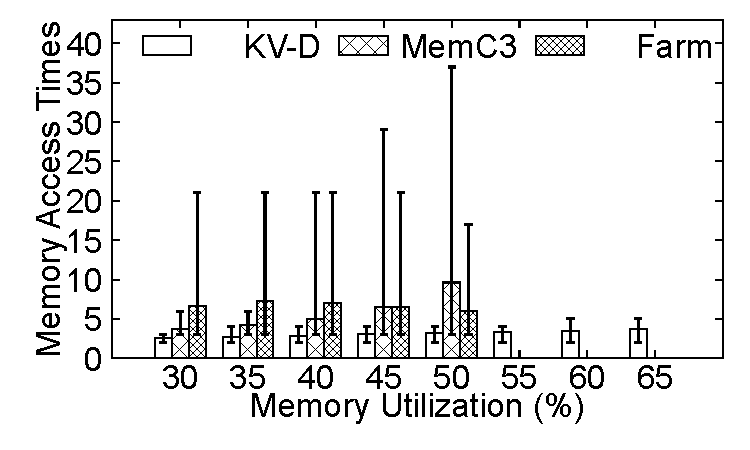
\includegraphics[width=.5\textwidth,page=1]{10B_put.pdf}}
	
	\vfill
	
	\subfloat[254B GET.\label{kvdirect:fig:mem-access-254-get}]
	{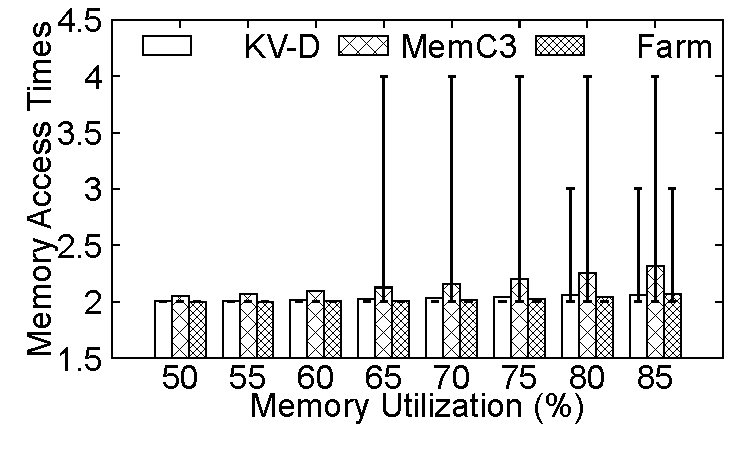
\includegraphics[width=.5\textwidth,page=1]{254B_get.pdf}}
	\subfloat[254B PUT.\label{kvdirect:fig:mem-access-254-put}]
	{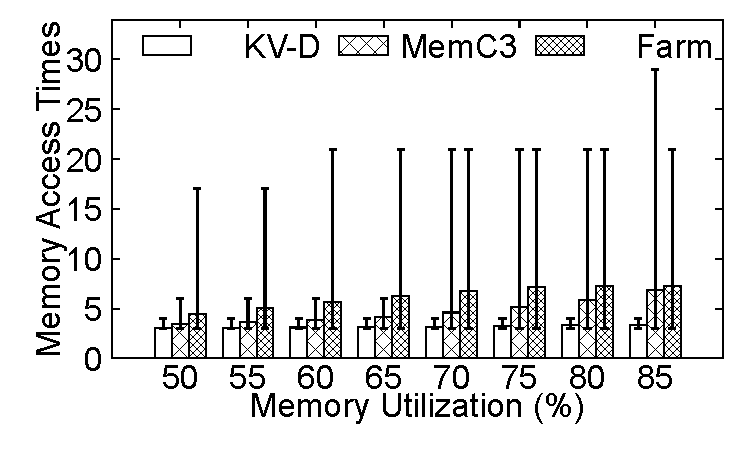
\includegraphics[width=.5\textwidth,page=1]{254B_put.pdf}}
	\caption{每个键值操作的内存访问次数。}
	\label{kvdirect:fig:mem-access-tput}
\end{figure}


对于内联键值,KV-Direct在每个GET上接近1个内存访问,在非极端内存利用率下每个PUT接近2个内存访问。
非内联键值的GET和PUT有一个额外的内存访问。
在高内存利用率下比较KV-Direct和链式跳房子哈希,跳房子哈希在GET中表现更好,但在PUT中表现更差。
虽然KV-Direct无法保证最坏情况下的DMA访问,但会在GET和PUT之间取得平衡。
布谷鸟哈希需要在GET上访问最多两个哈希槽,因此在大多数内存利用率下,KV-Direct具有更多的内存访问。
在高内存利用率下,布谷鸟哈希会导致每个PUT的内存访问时间出现大幅波动。



\subsection{Slab 内存分配器}
\label{kvdirect:sec:slab}

链式哈希槽和非内联键值需要动态内存分配。
为此,选择slab内存分配器\cite {bonwick1994slab}来实现每个分配和释放的$O(1)$平均内存访问。主slab分配器逻辑在主机CPU上运行,并通过PCIe与键值处理器通信。
Slab分配器将分配大小四舍五入到最接近的2的幂,称为\textit {slab 大小}。
它为每个可能的slab大小(32,64,\ldots,512字节)和全局 \textit {分配位图}维护\textit {空闲 slab 池},以帮助将小的空闲slab合并回更大的slab。
每个空闲slab池是一个\textit {slab 条目}数组,由一个地址字段和一个slab类型字段组成,表示slab条目的大小。
可以在网卡上缓存可用的slab池。缓存与批量的slab条目中的主机内存同步。通过批处理分摊,每次分配或解除分配需要少于0.07的DMA操作。
当一个小板坯池几乎是空的时,需要拆分较大的板坯。
因为slab类型已经包含在slab条目中,所以在\textit {slab 分割}中,slab条目只是从较大的池复制到较小的池,而不需要计算。
在slab条目中包括slab类型也可以节省通信成本,因为一个slab条目可能包含多个槽。

在重新分配时,slab分配器需要检查释放的slab是否可以与其邻居合并,需要至少一次读取和写入分配位图。
受垃圾收集的启发,建议\textit {懒惰 slab 合并}在一个slab池几乎为空时并且没有更大的slab池有足够的slab来拆分时批量合并空闲slab。


\begin{figure}[htbp]
	\centering
	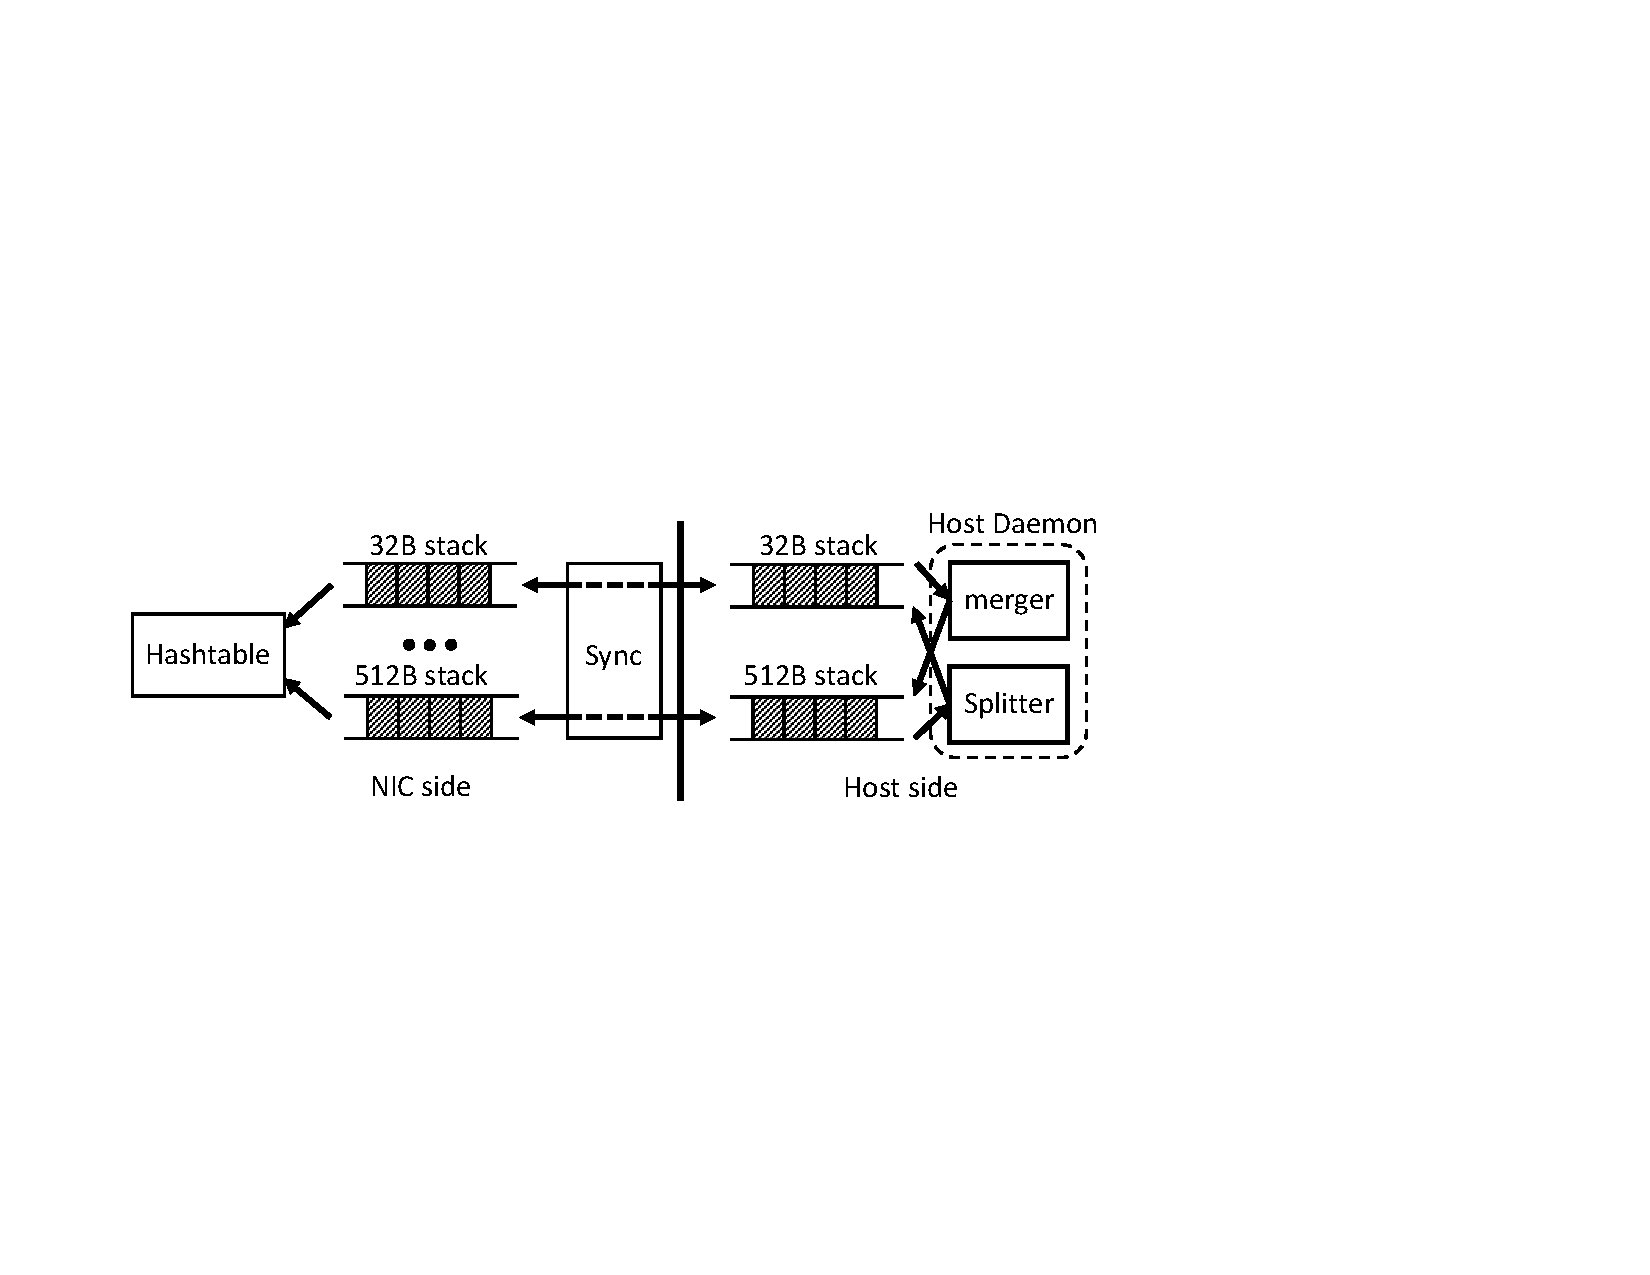
\includegraphics[width=.8\textwidth,page=1]{figure/cropped_slab.pdf}
	\caption{Slab 内存分配器。}
	\label{kvdirect:fig:slab}
	
\end{figure}

如图\ref {kvdirect:fig:slab}所示,对于每个slab大小,网卡上的slab缓存使用两个双端堆栈与主机DRAM同步。
对于网卡端双端堆栈(图\ref {kvdirect:fig:slab}中的左侧),左端由分配器和解除分配器弹出并推送,右端与左端同步通过DMA对应的​​主机端堆栈。
网卡监视网卡堆栈的大小,并根据高水位线和低水位线与主机堆栈同步。
主机守护进程定期检查主机端双端堆栈的大小。如果它高于高水印,则触发平板合并;当它低于低水印时,会触发平板分裂。
因为堆栈的每一端都是由网卡或主机访问的,并且在移动指针之前访问数据,所以不会发生竞争条件。

在本文中,每个slab条目是5个字节,DMA粒度是64个字节,因此每个slab操作的摊销DMA开销是$ 5/64 $。此外,当后续分配重新使用新释放的slab槽时,使用网卡上的堆栈而不是DMA。

\label{kvdirect:sec:slab-eval}


slab内存分配器的通信开销来自网卡访问主机内存中的可用slab队列。
为了维持每秒180M操作的最大吞吐量,在最坏的情况下,需要传输180M平板插槽,消耗720 MB / s PCIe吞吐量,即网卡的总PCIe吞吐量的5%。

slab内存分配器的计算开销来自主机CPU上的slab拆分和合并。
幸运的是,它们并不经常被调用。
对于具有稳定键值大小分布的工作负载,新释放的slab槽由后续分配重用,因此不会触发拆分和合并。

板坯分裂需要将连续的板坯条目从一个板坯队列移动到另一个板坯队列。当工作负载从大键值转换到小键值时,在最坏的情况下,CPU需要每秒移动90M板条目,这只占核心的10%,因为它只是连续的内存复制。

将自由平板槽合并到较大的槽是相当耗时的任务,因为它涉及用可能随机的偏移填充分配位图,因此需要随机存储器访问。
要对自由平板的地址进行排序并合并连续的平板,基数排序 \cite {satish2010fast} 可以比简单的位图更好地扩展到多个内核。
如图\ref {kvdirect:fig:slab-garbage-collection} 所示,将16 GiB向量中的所有40亿个空闲 slab 槽位合并在一个内核上需要30秒,或者在32个内核上使用基数排序仅需1.8秒 \cite{satish2010fast}。
虽然垃圾收集空闲 slab 槽位需要几秒钟,但它在后台运行而不会停止 slab 分配器,并且实际上仅在工作负载从小键值转换到大键值时触发。


\begin{figure}[t]
	\centering
	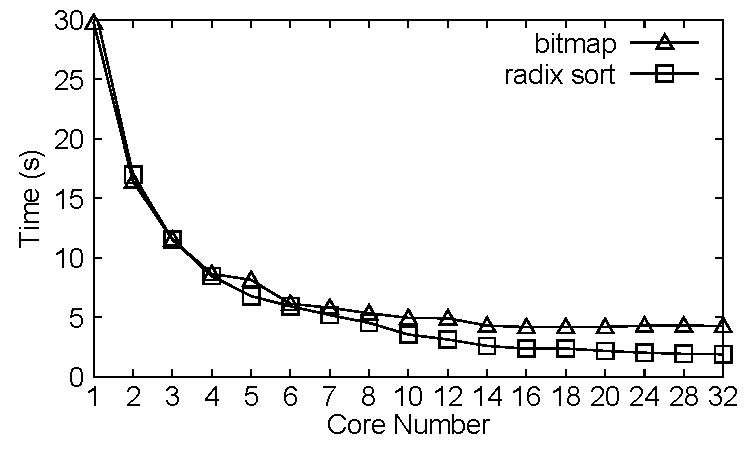
\includegraphics[width=0.6\textwidth]{slab-gc.pdf}
	\caption{合并 40 亿个 slab 槽位的时间开销。}
	\label{kvdirect:fig:slab-garbage-collection}
\end{figure}




\subsection{乱序执行引擎}
\label{kvdirect:sec:ooo}

\begin{figure}[htbp]
\centering
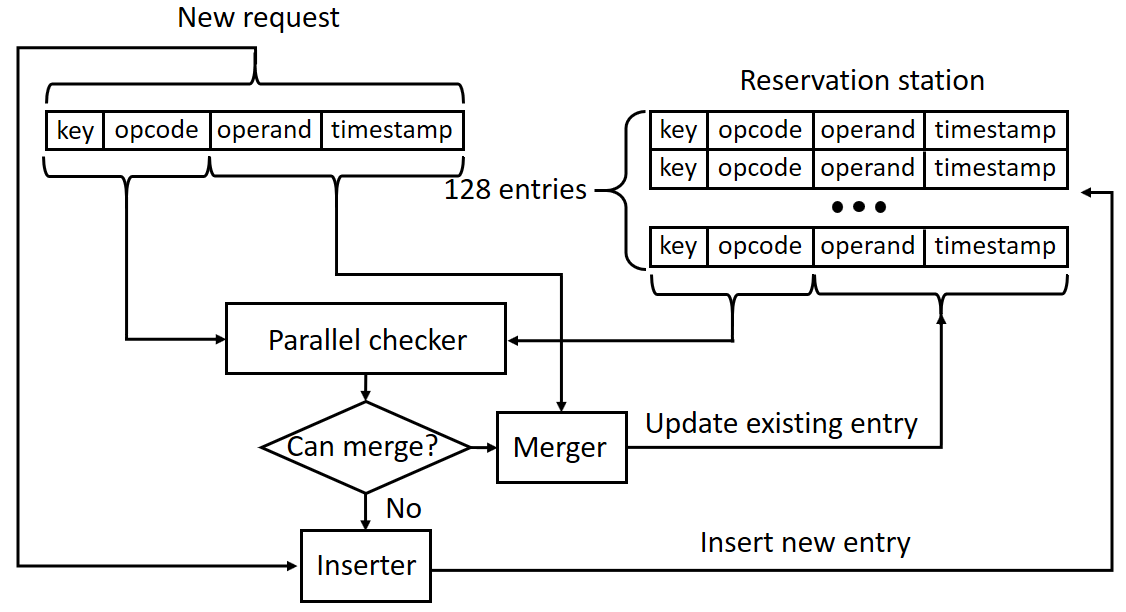
\includegraphics[width=.9\textwidth,page=1]{dynamic_scheduler.PNG}
\caption{乱序执行引擎。}
\label{kvdirect:fig:ooo-mem-access}
\end{figure}

在键值处理器中使用相同键的两个键值操作之间的依赖性将导致数据危险和管道停滞。
这个问题在单键原子中被放大,其中所有操作都是依赖的,因此限制了原子的吞吐量。
本节从计算机体系结构借用动态调度的概念,并实现\textit {保留站}(reservation station)来跟踪所有正在进行的键值操作及其\textit {执行上下文}。
为了使PCIe,DRAM和处理流水线饱和,需要多达256个正在执行的键值操作。
但是,并行比较256个16字节键将占用FPGA的40%逻辑资源。
相反,本节将键值操作存储在片上BRAM中的小哈希表中,由键的哈希索引。
键值操作可能具有相同的哈希值,因此可能存在误报,但它永远不会错过依赖关系。
具有相同哈希的操作在链中组织并顺序检查。
哈希冲突会降低链检查的效率,因此保留站包含1024个哈希槽,使哈希冲突可能性低于25%。

保留站不仅保留挂起的操作,还缓存\textit {数据转发}(data forwarding)的最新值。
当主处理流水线完成键值操作时,其结果返回给客户端,最新值被转发到保留站。
逐个检查相同哈希槽中的待定操作,并立即执行具有匹配键的操作并从保留站移除。
对于原子操作,计算在专用执行引擎中执行。
对于写入操作,将更新缓存的值。
执行结果直接返回给客户端。
在扫描从属操作链之后,如果更新了高速缓存的值,则向主处理管道发出PUT操作以进行高速缓存写回。
这种数据转发和快速执行路径使单键原子能够在每个时钟周期(180~Mops)内处理一次操作,消除了常用键在工作负载下的线头阻塞,并确保一致性,因为在同一个键上没有两个操作可以在主处理管道中同时进行。


\label{kvdirect:sec:ooo-eval}

本节通过比较吞吐量和在原子和长尾工作负载下使关键冲突管道停滞的简单方法,评估乱序执行的有效性。单面RDMA和双面RDMA \cite {kalia2016design}吞吐量也显示为基线。

如果没有此引擎,原子操作需要等待网卡中的PCIe延迟和处理延迟,在此期间无法执行对同一键的后续原子操作。
这使得单键原子吞吐量在图 \ref{kvdirect:fig:ooo-atomic} 中为0.94~Mops,与从RDMA 网卡测量的2.24~Mops一致 \cite {kalia2016design}。
RDMA 网卡的更高吞吐量可归因于其更高的时钟频率和更低的处理延迟。
对于无序执行,KV-Direct中的单键原子操作可以在峰值吞吐量下处理,即每个时钟周期一次操作。
在MICA \cite {lim2014mica} 中,单键原子吞吐量无法扩展到单个核心之外。
原子提取和添加可以扩展到 \cite {kalia2016design} 中的多个核心,但它依赖于原子之间的可交换性,因此不适用于非交换原子,如比较和交换。

随着无序执行,单键原子吞吐量提高了191倍,达到了180~Mops的时钟频率范围。
当原子操作在多个键之间均匀分布时,单向RDMA,双向RDMA和KV-Direct的吞吐量没有无序执行随着键的数量线性增长,但仍然远离键值的最佳吞吐量-直接。

图 \ref {kvdirect:fig:ooo-longtail} 显示了长尾工作负载下的吞吐量。
回想一下,当PUT操作使用相同的键找到任何正在进行的操作时,管道会停止。
长尾工作负载具有多个非常流行的键,因此具有相同流行键的两个操作很可能及时到达。
具有更高的PUT比率,更有可能的是,两个操作中的至少一个是PUT,因此触发流水线停顿。


\begin{figure}[htbp]
	\centering
	\subfloat[原子操作。\label{kvdirect:fig:ooo-atomic}]
	{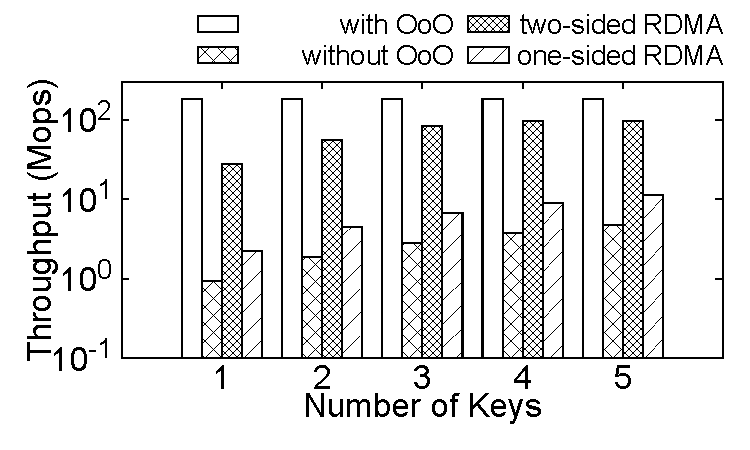
\includegraphics[width=.5\textwidth,page=1]{ooo_atomic.pdf}}
	\subfloat[长尾负载。\label{kvdirect:fig:ooo-longtail}]
	{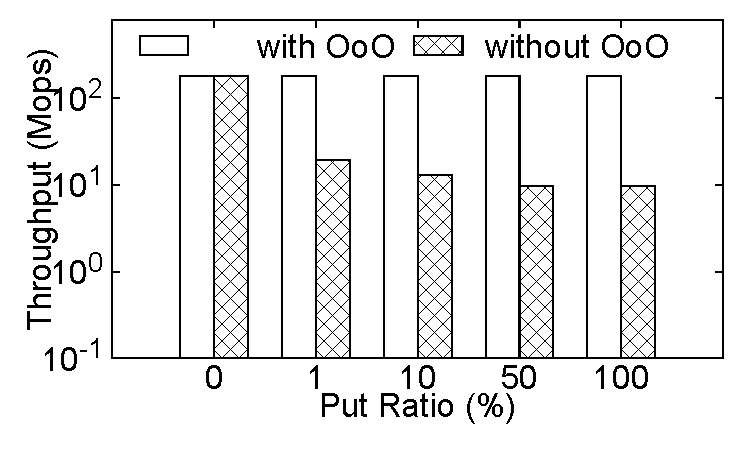
\includegraphics[width=.5\textwidth,page=1]{ooo_long-tail.pdf}}
	\caption{乱序执行引擎的效率。}
	\label{kvdirect:fig:ooo-eval}
\end{figure}



\subsubsection{DRAM 负载分配器}
\label{kvdirect:sec:dram-cache}

为了进一步减轻PCIe的负担,本节在PCIe和网卡板载DRAM之间调度内存访问。
网卡 DRAM具有4~GiB大小和12.8~GB / s的吞吐量,比主机DRAM(64~GiB)上的键值存储存储小一个数量级,并且比PCIe链路(14~GB / s)稍慢。
一种方法是将固定部分的键值存储放入网卡 DRAM中。但是,网卡 DRAM太小而无法承载大部分内存访问。
另一种方法是使用网卡 DRAM作为主机内存的缓存,由于网卡 DRAM的吞吐量有限,吞吐量会降低。


\begin{figure}[htbp]
	\centering
	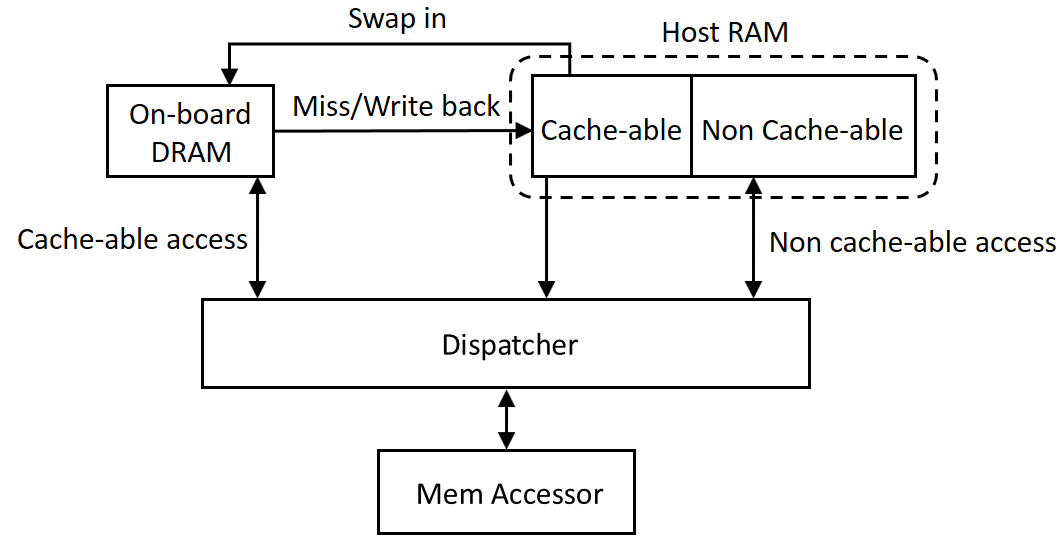
\includegraphics[width=0.8\textwidth,page=1]{load_balancer.PNG}
	\caption{DRAM 负载分配器。}
	\label{kvdirect:fig:cache}
\end{figure}


本节采用混合解决方案将DRAM用作主机内存中固定部分键值存储的缓存,如图\ref {kvdirect:fig:cache}所示。
可缓存部分由存储器地址的哈希确定,其粒度为64字节。选择哈希函数,使得哈希索引和动态分配的存储器中的地址具有可高速缓存的相同可能性。
整个键值存储内存中可缓存内存的部分称为\textit {负载分配比例}($ l $)。
使用更大的负载调度比$ l $,将更多负载分配给板载DRAM,并且缓存命中率$ h(l)$将增加。
假设缓存命中率可能是$ h(l)$。
为了平衡PCIe和板载DRAM上的负载,应优化负载调度比$ l $,使得:
$$\frac{l}{tput_{DRAM}} = \frac{(1-l) + l \cdot (1-h(l))}{tput_{PCIe}}$$

特别的,在均匀(uniform)负载下,令 $k$ 是板上 DRAM 大小和主机 键值 存储大小之比,则缓存命中率 $h(l) = \frac{\textnormal{cache size}}{\textnormal{cache-able memory size}} = \frac{k}{l}$,当 $k \leq l$ 时。
一致负载下的缓存并不高效。
在长尾负载(Zipf 分布)下,设 $n$ 是 键值 的总数,则大致上 $h(l) = \frac{\log (\textnormal{缓存大小})}{\log (\textnormal{可缓存部分大小})} = \frac{\log (kn)}{\log (ln)}$,当 $k \leq l$ 时。
在长尾工作负载下,1G语料库中1M缓存的缓存命中可能性高达0.7。
最优的 $l$ 可以得出数值解,将在 \S\ref{kvdirect:sec:different-nic} 中讨论。



一个技术挑战是在DRAM高速缓存中存储元数据,这需要额外的4个地址位和每64字节高速缓存行一个脏标志。
不需要缓存有效位,因为所有键值存储存储都由网卡专门访问。
为了存储每个高速缓存行的5个元数据位,将高速缓存行扩展到65个字节会由于未对齐访问而降低DRAM性能;将元数据保存在别处会使内存访问倍增。
相反,本文利用ECC DRAM中的备用位来进行元数据存储。
ECC DRAM通常每64位数据具有8个ECC位。
对于汉明码来纠正64位数据中的一位错误,只需要7个附加位。
第8个ECC位是用于检测双位错误的奇偶校验位。
当以64字节粒度和对齐方式访问DRAM时,每64B数据有8个奇偶校验位。
本文将奇偶校验检查粒度从64个数据位增加到256个数据位,因此仍然可以检测到双位错误。这允许了6个额外的位,可以保存地址位和脏标志。


图 \ref {kvdirect:fig:cache-tput} 显示了仅在使用PCIe的基线上DRAM负载调度的吞吐量改进。
在统一工作负载下,DRAM的缓存效果可以忽略不计,因为它的大小仅为主机键值存储内存的6%。
在长尾工作负载下,大约30%的内存访问由DRAM缓存提供。 总的来说,95%和100%GET的内存访问吞吐量实现了180 Mops的时钟频率限制。
但是,如果简单地将DRAM用作高速缓存,则吞吐量将受到不利影响,因为DRAM吞吐量低于PCIe吞吐量。


\begin{figure}[htbp]
	\centering
	{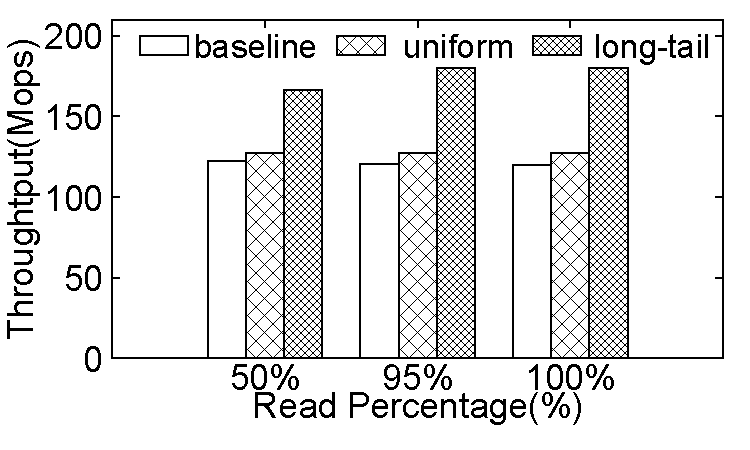
\includegraphics[width=.5\textwidth,page=1]{load_balancer.pdf}}
	\caption{负载分派下的 DMA 吞吐量(固定负载分派比例为 0.5)。}
	\label{kvdirect:fig:cache-tput}
\end{figure}



\subsection{向量操作译码器}

在整个键值处理器设计中,将批处理视为在一个存储桶中获取多个哈希槽,使自由slab队列与主机内存同步,懒惰拆分和slab槽合并以及依赖键值操作的数据转发的通用原则。
批处理通过将控制平面开销分摊到多个数据平面有效负载来提高性能。
与PCIe相比,网络是一种更加稀缺的资源,具有更低的带宽(5~GB / s)和更高的延迟(2~$\mu$s)。
以太网上的RDMA写数据包有88字节的报头和填充开销,而PCIe TLP数据包只有26字节的开销。
这就是以前基于FPGA的键值存储 \cite{blott13hotcloud,blott2015scaling} 没有使PCIe带宽饱和的原因,尽管它们的哈希表设计效率低于KV-Direct。
这需要在两个方面进行\textit {客户端批处理}:在一个数据包中批量处理多个键值操作,并支持向量操作以实现更紧凑的表示。为此,在键值引擎中实现了一个解码器,从单个RDMA数据包中解压缩多个键值操作。
观察到许多键值具有相同的大小或重复值,键值格式包括两个标志位以允许复制键和值大小,或者包中的先前键值的值。
幸运的是,许多重要的工作负载(\textit {例如图遍历,参数服务器})可以批量发布键值操作。
展望未来,如果可以使用更高带宽的网络,则无需批量处理。


为了评估KV-Direct中向量操作的效率,
表 \ref {kvdirect:tab:vec_throughput}将原子向量增量的吞吐量与两种替代方法进行比较:
(1)如果每个元素都存储为唯一键,则瓶颈是传输键值操作的网络。
(2)如果向量存储为大的不透明值,则向客户端检索向量也会使网络瘫痪。
此外,表 \ref {kvdirect:tab:vec_throughput} 中的两个备选方案不能确保向量内的一致性。 添加同步会产生进一步的开销。


\begin{table}[htbp]
	\centering
	\caption{向量操作的吞吐量 (GB/s)。}
	\label{kvdirect:tab:vec_throughput}
	\small
		\begin{tabular}{|l|r|r|r|r|r|}
			\hline
			向量大小 (字节)              & 64    & 128   & 256   & 512   & 1024  \\ \hline
			向量更新(有返回)    & 11.52 & 11.52 & 11.52 & 11.52 & 11.52 \\ \hline
			向量更新(无返回) & 4.37  & 4.53  & 4.62  & 4.66  & 4.68  \\ \hline
			每个元素一个键         & 2.09  & 2.09  & 2.09  & 2.09  & 2.09  \\ \hline
			取回客户端处理             & 0.03  & 0.06  & 0.12  & 0.24  & 0.46  \\ \hline
		\end{tabular}
\end{table}




KV-Direct客户端在网络数据包中打包键值操作,以减轻数据包报头开销。
图 \ref {kvdirect:fig:eval-network-batching} 表明,网络批处理可将网络吞吐量提高4倍,同时保持网络延迟低于3.5 $\mu$s。


\begin{figure}[htbp]
	\centering
	\subfloat[吞吐量。\label{kvdirect:fig:network-batching-bw}]
	{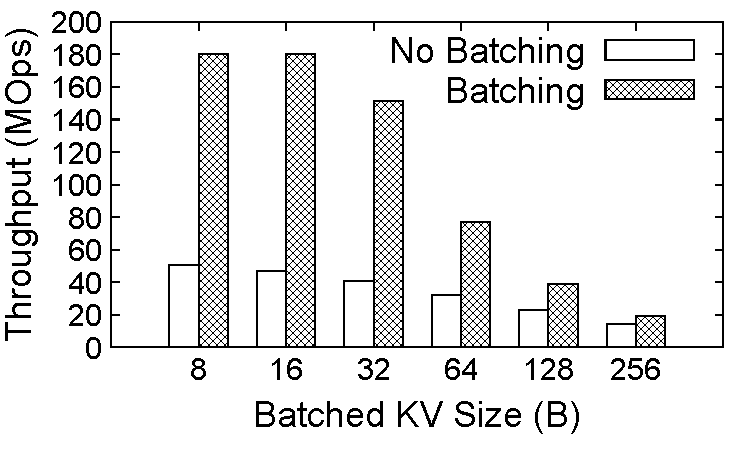
\includegraphics[width=.5\textwidth,page=1]{net_batching_bw.pdf}}
	\subfloat[延迟。\label{kvdirect:fig:network-batching-lat}]
	{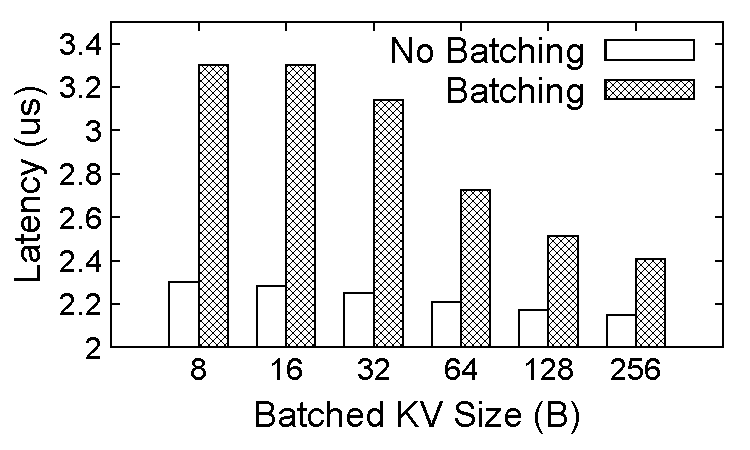
\includegraphics[width=.5\textwidth,page=1]{net_batching_lat.pdf}}
	\caption{网络批量化的效率。}
	\label{kvdirect:fig:eval-network-batching}
\end{figure}

\subsection{网络协议与客户端}


\egg{
\subsubsection{Congestion Avoidance}
\label{kvdirect:sec:congestion-avoidance}

In addition to throughput, another important factor is latency.
From the client's perspective, the 键值 processor is a path with multiple bottlenecks and buffers, \eg, PCIe and DRAM access.
If all buffers in the 键值 processor are filled up, the GET latency would exceed 10~$\mu$s.
To mitigate the bufferbloat problem, we implement a congestion avoidance logic to limit the number of in-flight 键值 operations \textit{inside the 键值 processor}.
The 键值 processor maintains a \textit{键值 operation window} and leverages credit-based flow control mechanism in RDMA to back-pressure 键值存储 clients.
To adapt 键值 operation window size to the workload, we measure the running average of 键值 processing delay and adjust the window size according to TCP Vegas congestion avoidance algorithm~\cite{brakmo1995tcp}.
%We use delay as the congestion signal instead of ECN, because the queues whose sizes are hard to measure.
}
